\documentclass[12pt]{article}

% Specify document formatting.
\renewcommand{\baselinestretch}{1.0} 
\usepackage[top=2.5cm,bottom=2.5cm,inner=4cm,outer=2.5cm,twoside]{geometry}
\usepackage{fancyhdr} \usepackage{pdfpages} \usepackage[nottoc,notlof,notlot,numbib]{tocbibind}

% Change section title font size to 12.
\usepackage[none]{hyphenat} \usepackage{sectsty}
\sectionfont{\fontsize{12}{10}\selectfont}
\subsectionfont{\fontsize{12}{10}\selectfont}
\subsubsectionfont{\fontsize{12}{10}\selectfont}

\usepackage{fontspec}
\setmainfont{Times New Roman}

\usepackage{amsmath} \usepackage{graphicx} \usepackage{microtype} \usepackage{float}
\usepackage[hidelinks]{hyperref} \usepackage{cleveref}
\usepackage{siunitx} \usepackage{gensymb} \usepackage{enumitem}
\usepackage{tabularx} \usepackage{booktabs} \usepackage{adjustbox} \usepackage{makecell}
\usepackage[style=ieee]{biblatex} \addbibresource{zotero.bib}

\usepackage{listings}

\setcounter{bottomnumber}{1}
\renewcommand\bottomfraction{10.0}

\begin{document}
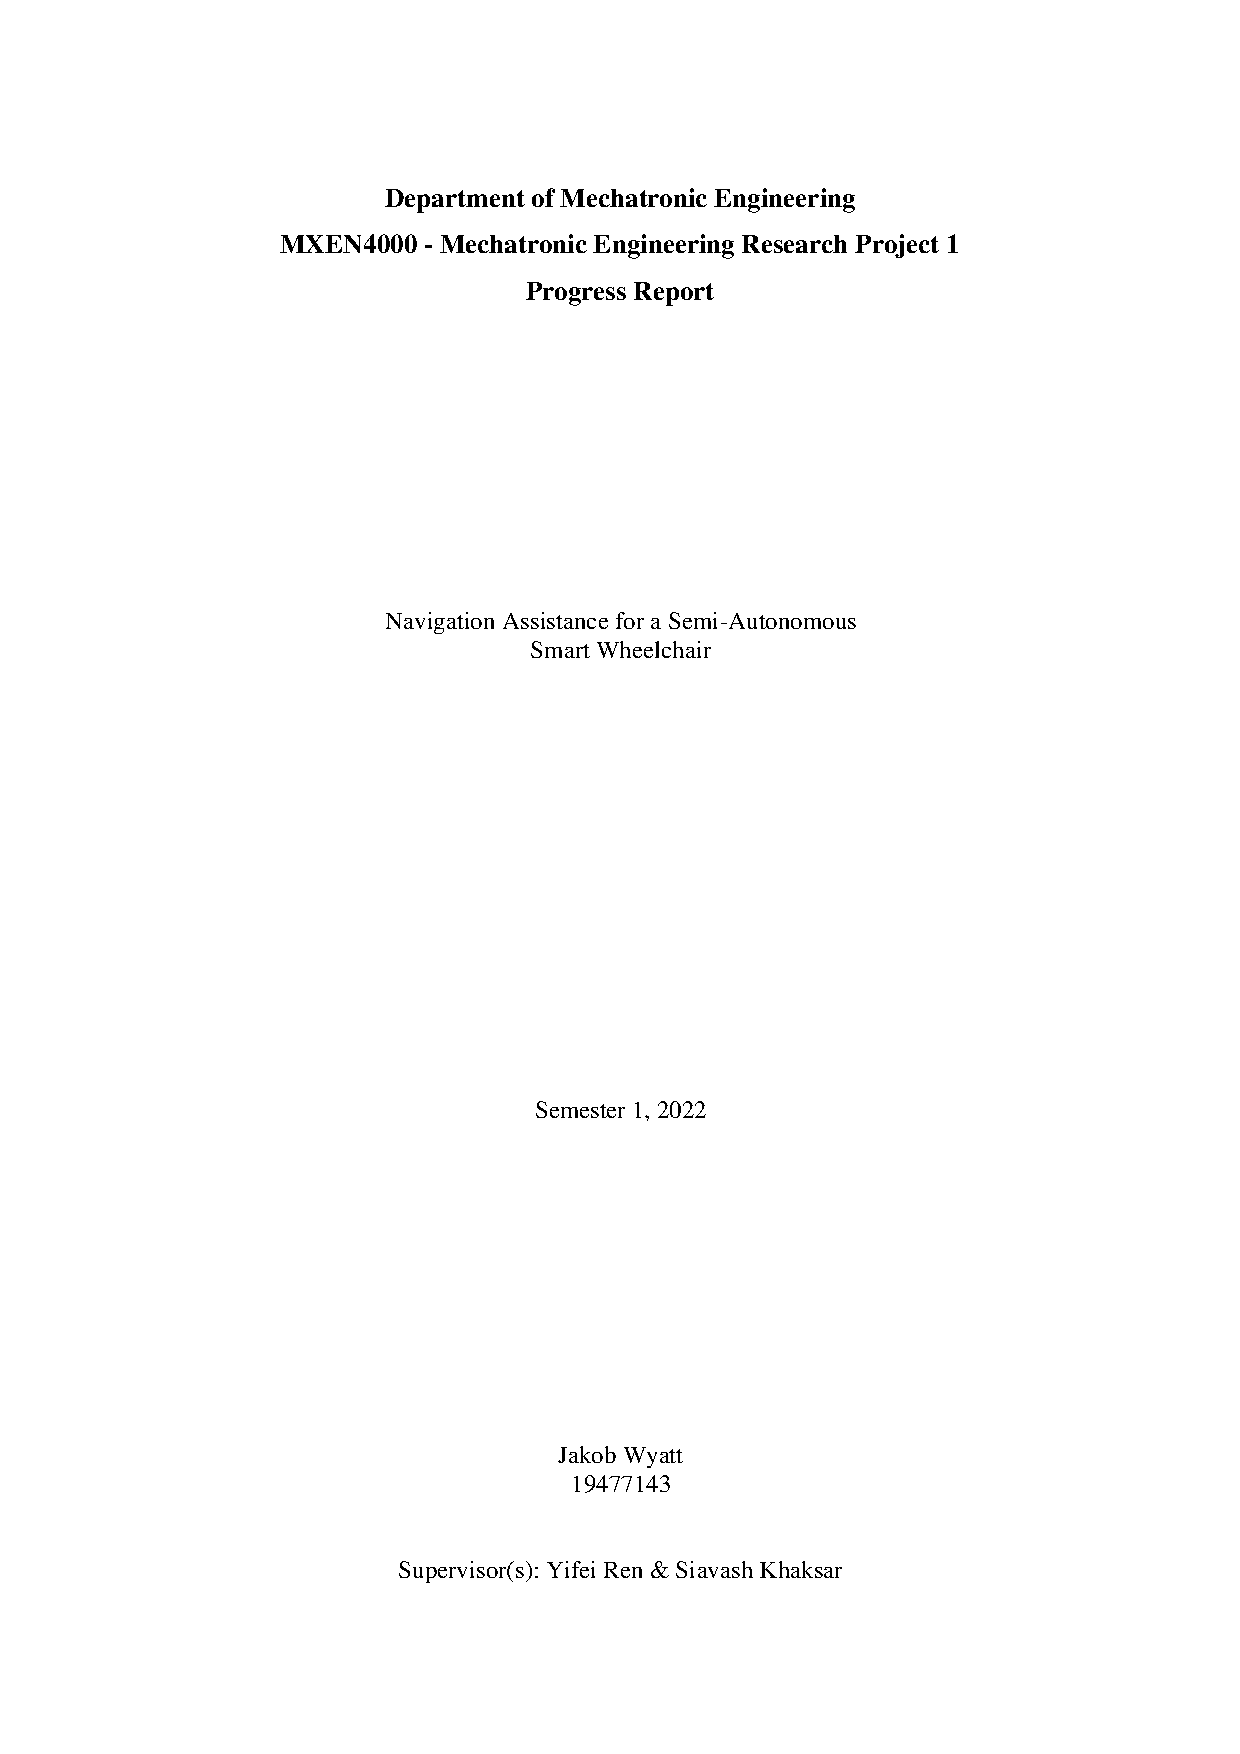
\includepdf{title.pdf}
\thispagestyle{empty}
\pagebreak

\pagenumbering{roman}
\section*{Abstract}
%\addcontentsline{toc}{section}{Abstract}
\pagebreak

\renewcommand{\contentsname}{Table of Contents}
\tableofcontents
\pagebreak
\listoffigures
\listoftables
\pagebreak

\pagenumbering{arabic}


% Figures to add:
% Unet network


\section{Introduction}
Many people with motor disabilities rely on wheelchairs for movement, and
powered wheelchairs have enabled greater independance for people with disability.
Despite the huge benefit powered wheelchairs have granted,
the use of this technology can be inaccessible or unsafe for people
with amyotrophic lateral sclerosis (ALS) or vision impairment,
who may be unable to use a joystick or see their environment clearly.


\subsection{Aims}
The aim of this research is to develop a semi-autonomous smart wheelchair system.
This research is done in collaboration with Glide, a WA wheelchair manufacturer,
who have provided an existing powered wheelchair (CentroGlide) to use as a base
for this functionality (\cref{fig:wheelchair_reclined}). By developing assistive technology for the wheelchair,
the user is granted greater mobility, confidence, and independence.

\begin{figure}[H]
    \centering
    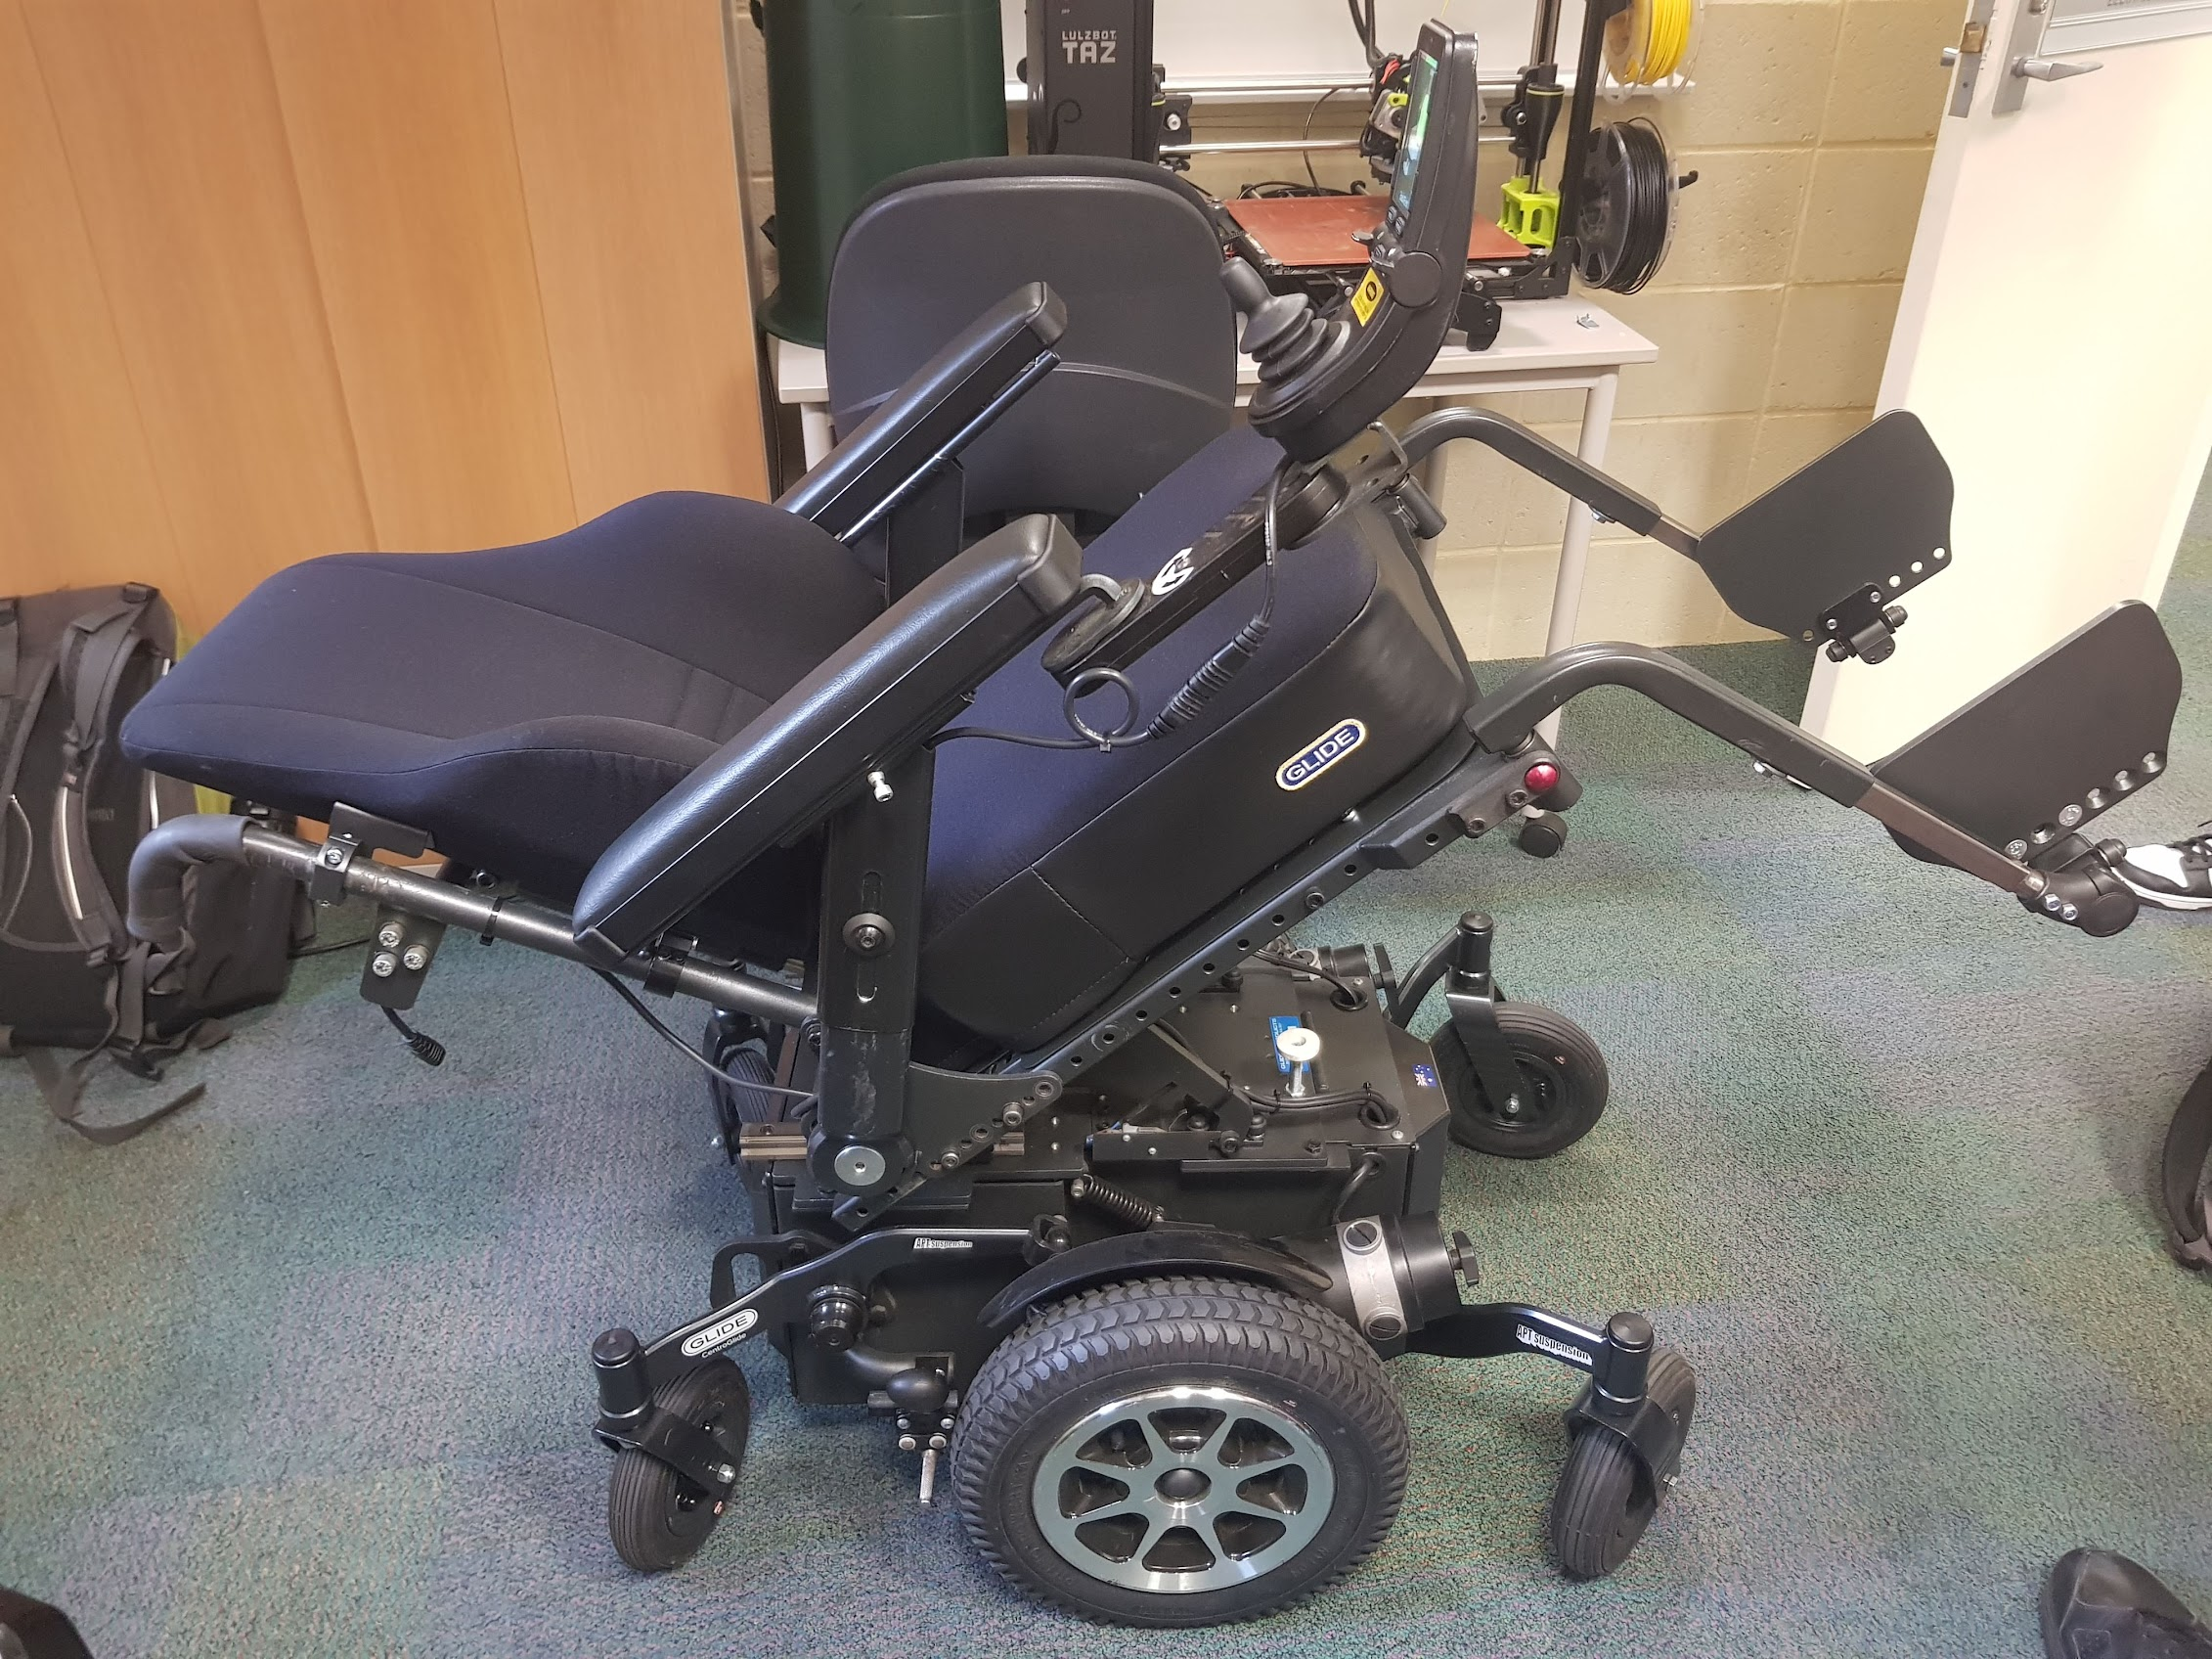
\includegraphics[width=0.6\linewidth]{images/wheelchair_reclined.jpg}
    \caption{CentroGlide in Reclined Configuration}
    \label{fig:wheelchair_reclined}
\end{figure}

\pagebreak
\subsection{Problem Definition}
There are multiple engineering research project students who are part of this team,
working on elements such as controller design, navigation assistance, and object detection.
This work specifically focuses on pathway assistance, which identifies suitable
paths for the wheelchair to drive on. If a user unintentionally drives off their desired path,
this can lead to uneven terrain and possibly falling from the wheelchair.
By guiding the user along a path, these safety issues can be mitigated.

Emphasis is placed on the 'semi-autonomous' aspect of the wheelchair.
An important requirement of this project is that the user still
has control over their wheelchair, and can override any autonomous functionality
if required. If the smart wheelchair system mistakenly detects an obstacle,
the users mobility should not be compromised.

Another requirement of the system is that any sensors mounted to the wheelchair
should not impede the users comfort or the wheelchairs manouverability.
Many wheelchair users have specific requirements for wheelchair seat adjustments,
to avoid pressure sores and discomfort. \Cref{fig:wheelchair_reclined} shows the
wheelchair configuration when fully reclined, demonstrating that some sensor mounting locations
are infeasible.

The smart wheelchair system should also be commercially viable - high-cost
components and sensors are infeasible. Internet connectivity should not be a requirement
for the system to operate either - the round trip time required to communicate with a server
would compromise the safety of a user. Because of this, all processing is performed locally
on the wheelchair.

\pagebreak





\section{Literature Review}
%Smart wheelchairs are wheelchairs with additional sensors and computers,
%enabling greater usability and safety. This can come in the form of alternative input methods,
%such as eye-gaze tracking \cite{eidNovelEyeGazeControlledWheelchair2016} or using a brain-computer
%interface \cite{kaufmannBraincomputerInterfaceBased2014} to control the wheelchair. For people with vision impairment,
%haptic feedback \cite{kondoNavigationGuidanceControl2008}\cite{vanderpoortenPoweredWheelchairNavigation2012}
%has been used to improve awareness of the surrounding environment and make indoor navigation safer.


\subsection{Sensors and Hardware}
%To percieve the environment, the wheelchair should be fitted with various sensors and
%a compute element to process the sensors output.

\subsubsection{Sensor Types}
Smart wheelchairs have used a varied range of sensor types to percieve the surrounding environment.
RGB-D stereo cameras have been widely used in the field \cite{wangS2P2SelfSupervisedGoalDirected2021}\cite{wangSelfSupervisedDrivableArea2019}\cite{jainAutomatedPerceptionSafe2014},
alongside 2d Lidar \cite{scudellariSelfdrivingWheelchairsDebut2017} and ultrasonic sensors \cite{levineNavChairAssistiveWheelchair1999}.
Self-driving cars built by companies such as Tesla and Waymo
use cameras, mmWave Radar, and 3d Lidar to avoid traffic and pedestrians \cite{karpathyTeslaAIDay2021}.

Selecting a sensor to use is not necessarily an either-or decision. Sensor fusion algorithms such as
the Extended Kalman Filter (EKF) or Unscented Kalman Filter (UKF) \cite{wanUnscentedKalmanFilter2000} allow
outputs from multiple sensors to be used together to improve their accuracy. Additionally, sensors can
be used for different applications on the smart wheelchair - a stereo camera could be used to sense the surrounding environment
while an inertial measurement unit (IMU) could be used for wheelchair odometry.
\Cref{table:sensor_options} gives a comparison of several available sensor types,
taking into account factors such as resolution, cost, and accuracy.

\begin{table}[H]
    \centering
\begin{adjustbox}{width=\textwidth}
    \begin{tabular}{c c c}
    \toprule
    Sensor & Advantages & Disadvantages \\
    \midrule
    RGB-D Stereo Camera & Very high resolution & Low field of view (FOV) \\
    mmWave Radar & High accuracy & Low resolution \\
    3D Lidar & High resolution and accuracy & Very high cost \\
    2D Lidar & High FOV and accuracy & Only detects obstacles within the same plane \\
    Ultrasonic sensor & Low cost & One-dimensional \\
    \bottomrule
    \end{tabular}
\end{adjustbox}
    \caption{Sensor Comparisons}
    \label{table:sensor_options}
\end{table}

% Description of different sensor types?

\subsubsection{RGB-D Cameras}
One advantage RGB-D cameras have over alternative sensors is high RGB resolution,
allowing them to utilize advances in machine learning and computer vision.
Sensors such as LIDAR may fail at path detection, as path markings
cannot be detected.

When comparing these cameras, factors such as package size,
field of view, and depth accuracy are important to consider due to the available
mounting points on the wheelchair. Several commercial options are compared in \Cref{table:stereo_camera}
- all of the listed units come with an integrated IMU.

\begin{table}
    \centering
\begin{adjustbox}{width=\textwidth}
    \begin{tabular}{c c c c c c}
    \toprule
    Name & Type & Cost (AUD)\footnotemark[1] & Dimensions (mm) & FOV (Horizontal, Vertical, Depth) & Operating Range (m) \\
    \midrule
    Stereolabs Zed Mini \cite{stereolabsZEDMiniCamera2018} & Passive & \$595 & $124.5\times 30.5\times 26.5$ & $90\degree\times 60\degree\times 100\degree$ & 0.1-15\\
    Stereolabs Zed 2 \cite{stereolabsZEDCameraSDK2019} & Passive & \$670 & $175\times 30\times 33$ & $110\degree\times 70\degree\times 120\degree$ & 0.3-20 \\
    Intel RealSense D455 \cite{intelIntelRealSenseProduct2022} & Active IR (Stereo) & \$595 & $124\times 26\times 29$ & $90\degree\times 65\degree\times 87\degree$ & 0.6-6 \\
    Microsoft Azure Kinect DK \cite{microsoftAzureKinectDK2021} & Active IR (Time of Flight)\footnotemark[2] & \$595 & $103\times 39\times 126$ & $75\degree\times 65\degree\times 75\degree$ & 0.5-3.86 \\
    \bottomrule
    \end{tabular}
\end{adjustbox}
    \caption{Stereo Camera Options}
    \label{table:stereo_camera}
\end{table}

\footnotetext[1]{Costs are taken at RRP with an exchange rate of 1 AUD = 0.74 USD}
\footnotetext[2]{The Microsoft Azure Kinect DK has multiple operating modes which tradeoff between FOV, operating range, and resolution. The \texttt{NFOV unbinned} mode was compared, which provides good tradeoff between operating range and resolution.}

A caveat of the Stereolabs products is that they require a seperate CUDA enabled GPU (manufactured by Nvidia) to generate the point-cloud
and RGB-D image. In contrast, the Kinect DK only requires a CPU for processing, while the Intel RealSense performs processing onboard
and requires a USB-C 3.1 interface to communicate.

\subsubsection{Compute Element}
A compute element inside a semi-autonomous driving system generally consists of several components -
a microcontroller to process user inputs and
send signals to the motors, a general purpose computer to run pathfinding algorithms and log information,
and an AI accelerator to improve performance of on-board machine learning (ML) algorithms.

AI accelerators use specialized hardware to perform operations common in ML algorithms (such as matrix multiplication
and convolution) more efficiently than a CPU can. GPUs have been used widely for this application, however their high
power usage is infeasible for some applications. Embedded AI accelerators aim to provide greater power efficiency
at the cost of specialization.

Machine learning models often use mixed-precision (FP16) datatypes to store weights while training. Although improving the accuracy
of the model, FP16 datatypes are slow to manipulate during inference. Model quantization \cite{jacobQuantizationTrainingNeural2017} is a process where this FP16 datatype is replaced with an
INT8 datatype (using a scaling factor and bias) after training.
This gives a large speed improvement, while only losing a small amount
of model accuracy.
For this reason, modern AI accelerators focus on the performance of INT8 operations (TOPS, $10^9$ operations per second),
whereas earlier accelerators state the performance of FP16 operations (TFLOPS, $10^9$ floating-point
operations per second).

The Nvidia Jetson and Google Coral products are both popular options for embedded AI acceleration. These accelerators are compared
in \Cref{table:compute_element} alongside a gaming GPU. 

\begin{table}[H]
    \centering
\begin{adjustbox}{width=\textwidth}
    \begin{tabular}{c c c c c c}
    \toprule
    Name & Cost (AUD)\footnotemark[1] & Release Year & Speed & Power & Notes \\
    \midrule
    Nvidia Jetson Nano \cite{nvidiaJetsonNanoSystemonModule2019} & \$150 & Early 2019 & 0.5 TFLOPS (FP16) & 10 W & - \\
    Nvidia Jetson Xavier NX \cite{nvidiaJetsonXavierNX2019} & \$595 & Late 2019 & 21 TOPS (INT8) & 20 W & - \\
    Nvidia RTX 2080 \cite{nvidiaTuringGPUArchitecture2018} & \$1040 & 2018 & \makecell{80.5 TFLOPS (FP16)\\161.1 TOPS (INT8)} & 215 W & Doesn't include single-board computer \\
    Google Coral Edge TPU \cite{googlecoralCoralDevBoard2020} & \$190 & 2020 & 4 TOPS (INT8) & 2 W & Only supports TensorFlow Lite \\
    \bottomrule
    \end{tabular}
\end{adjustbox}
    \caption{AI Accelerator Options}
    \label{table:compute_element}
\end{table}

\pagebreak
\subsection{Scene Understanding}
Scene understanding is a broad field, and involves using computer vision methods
on visual or spatial data to gain better knowledge about the surrounding environment.
Convolutional Neural Networks (CNNs) are commonly used for this application, as they
are able to exploit the local nature of image features to reduce the number of required computations.

\subsubsection{Image Classification}
Image classification is a core problem within this field, and involves identifying the
subject of an image (such as an animal or object).
AlexNet \cite{krizhevskyImageNetClassificationDeep2012}, based on the earlier digit-recognition CNN LeNet-5
\cite{lecunGradientbasedLearningApplied1998}, was one of the first deep CNNs
applied to this problem. AlexNet was trained on the large ImageNet dataset \cite{jiadengImageNetLargescaleHierarchical2009},
which consists of 15M images and 22K categories,
and achieved an error of only 15.3\% on a 1000 class subset. The underlying architecture uses a series of 5 convolutional
layers and 3 fully connected layers, which can be seen in \cref{fig:alexnet_architecture}.

\begin{figure}[bp]
    \centering
    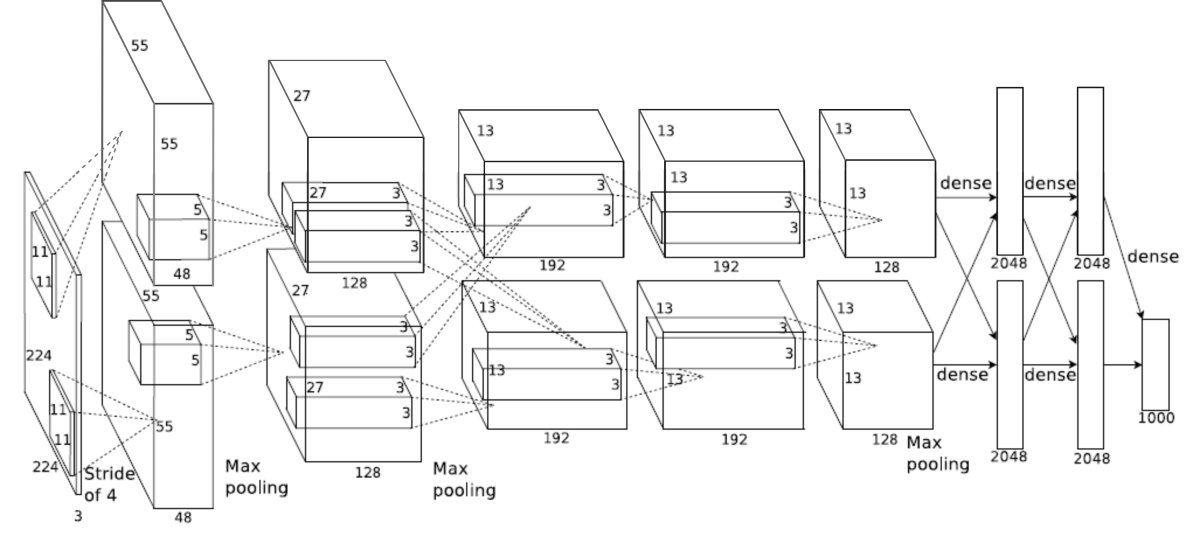
\includegraphics[width=0.8\linewidth]{images/alexnet_architecture.png}
    \caption{Architecture of the AlexNet image classification network. Reproduced from Krizhevsky et al. \cite{krizhevskyImageNetClassificationDeep2012})}
    \label{fig:alexnet_architecture}
\end{figure}

Neural network architectures have become deeper and more accurate over time, enabled by both
growth in computational power and dataset size. VGG-16 \cite{simonyanVeryDeepConvolutional2014}
and GoogLeNet \cite{szegedyGoingDeeperConvolutions2014}
are 16 and 22 layers deep respectively, and approached
human performance on the ImageNet dataset. ResNet \cite{heDeepResidualLearning2016} is up to 156 layers deep,
and exceeds human performance at image classification with an error of 3.57\%.
ResNet uses a 'skipping' architecture to improve network training, where the output of a layer relies directly on
the input of a previous layer.

\begin{figure}[bp]
    \centering
    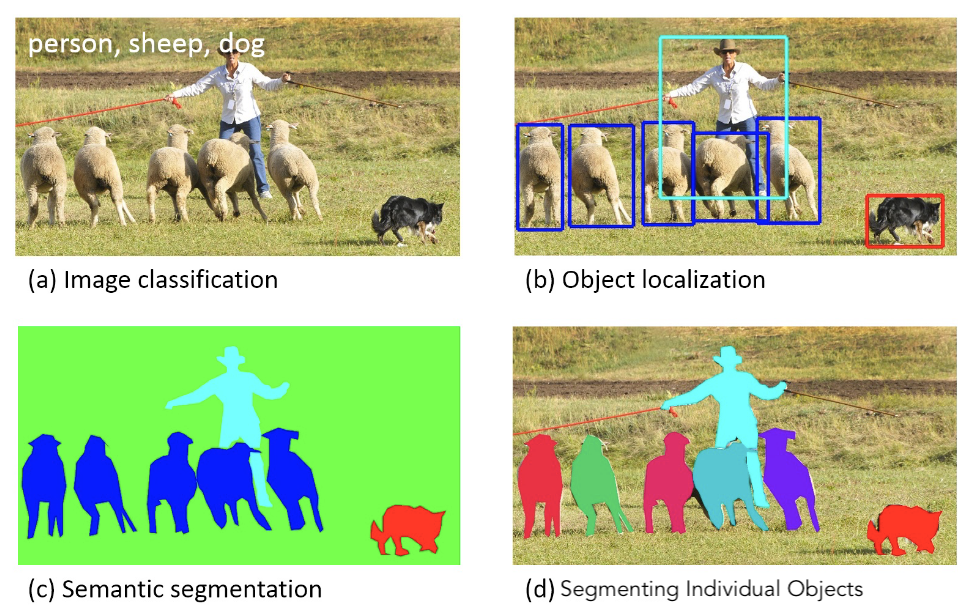
\includegraphics[width=0.6\linewidth]{images/classification_types.png}
    \caption{Types of Classification in Machine Vision. Reproduced from Lin et al. \cite{linMicrosoftCOCOCommon2014})}
    \label{fig:classification_types}
\end{figure}

\subsubsection{Object Localization}
Object localization is another core problem within this field, and involves identifying the location of objects within an image
as well as classifying them. Object localization can be used on a semi-autonomous wheelchair to identify
a pedestrian or obstacle within the environment. R-CNN \cite{girshickRichFeatureHierarchies2013} was one of the
first object classification models which utilized convolutional networks, by identifying potential bounding boxes
and running an image classifier on these bounding boxes. Fast and Faster R-CNN \cite{girshickFastRCNN2015}\cite{renFasterRCNNRealTime2015}
improved the speed of this model by running an image classifier backbone once on the entire image, and using a CNN to improve
identification of bounding boxes. Pascal VOC \cite{everinghamPascalVisualObject2009} and MS COCO \cite{linMicrosoftCOCOCommon2014}
are datasets which are commonly used to evaluate object classification models.

YOLO (You Only Look Once) \cite{redmonYouOnlyLook2015}\cite{redmonYOLO9000BetterFaster2016}\cite{redmonYOLOv3IncrementalImprovement2018}\cite{bochkovskiyYOLOv4OptimalSpeed2020}
is another object classification model which focuses on improving the speed of the model. In particular, YOLOv4 \cite{bochkovskiyYOLOv4OptimalSpeed2020}
reaches over 60 FPS (frames per second) on the Tesla V100, which enables its use in real time applications such as autonomous driving and security camera footage. % RCNN and YOLO
YOLO divides an image into an $S\times S$ grid, and uses a single convolutional network to output both bounding box predictions and
image classification for each grid square. Low-probability and overlapping bounding boxes are then removed before the final output.
%YOLOv4 uses a backbone-neck-head architecture

\subsubsection{Semantic Segmentation}
Semantic segmentation involves labelling each pixel of an object, rather than drawing a bounding box around the entire object.
This technique is often used in medical applications, where different components of a scan need to be labelled.
Another application semantic segmentation can be used for is drivable area detection, as a bounding box would not be able to cleanly
identify a road or kerb. \Cref{fig:classification_types} compares the output of semantic segmentation to image classification and object localization.

Most semantic segmentation algorithms use an encoder-decoder architecture, where information about the image is encoded into a small feature space.
This feature space is then decoded back to the size of the original image using deconvolutional layers to obtain the segmented output.
Encoding is typically done using a pretrained model backbone, such as ResNet. By avoiding model retraining and making use of
existing classifier backbones, the computational power required to evaluate a model is reduced significantly.
An issue with this architecture is that the resulting image can be low quality, as the image encoding is low resolution.
U-net \cite{ronnebergerUNetConvolutionalNetworks2015} is a semantic segmentation network which helps to rectify this issue,
by using higher resolution features during deconvolution.
This makes the segmented output sharper and more accurate.

Another semantic segmentation algorithm is DeepLab \cite{chenSemanticImageSegmentation2014}\cite{chenDeepLabSemanticImage2016}\cite{chenRethinkingAtrousConvolution2017}.
DeepLab uses atrous convolution (otherwise known as dilated convolution), which is a type of convolution which widens the FOV of a convolutional layer.
It does this by leaving gaps in the convolutional layer, as illustrated in \cref{fig:atrous_convolution}.
By widening the FOV of each convolution, less downscaling is required during encoding. By encoding the image in a much higher resolution feature space,
the segmented output is more accurate.
To obtain the segmented output, a technique called atrous spatial pyramid pooling (ASPP) is used. ASPP samples the feature space at different
scales using atrous convolution to classify each pixel in the image.
These techniques improve both the accuracy and speed of the network - DeepLabv3 obtained 86.9\% accuracy on the PASCAL VOC 2012 test set.

\begin{figure}[bp]
    \centering
    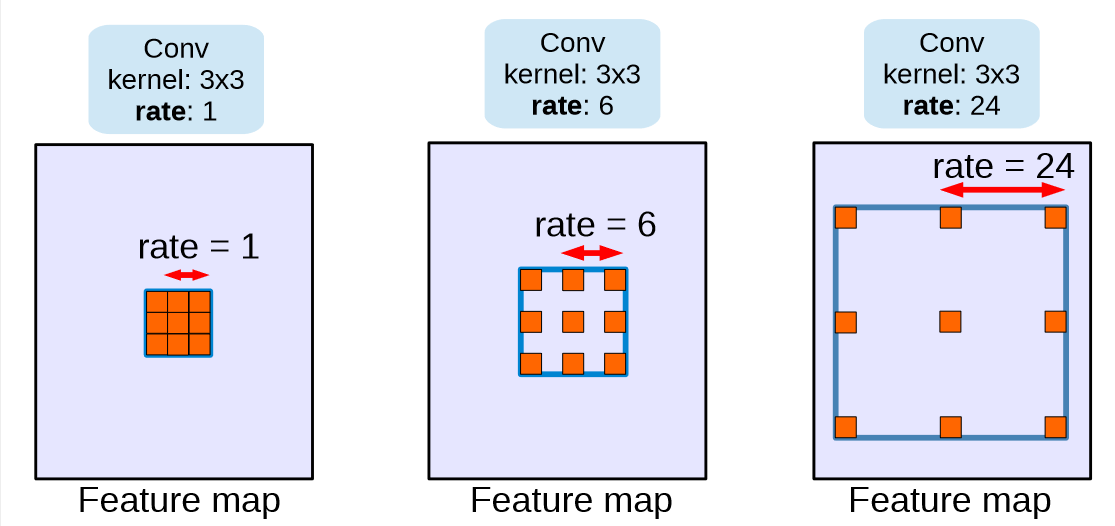
\includegraphics[width=0.6\linewidth]{images/atrous_convolution.png}
    \caption{Atrous convolution with a 3x3 kernel, showing increasing FOV. Reproduced from Chen et al. \cite{chenRethinkingAtrousConvolution2017})}
    \label{fig:atrous_convolution}
\end{figure}
% U-net, deepnet

% classification, localization, segmentation, video, datasets
% SLAM, mapping, hybridnet, etc.

\pagebreak
\subsection{Assistive Control}
Once an understanding of the 3d scene has been built, the user can be navigated through the environment.
The surrounding environment is generally represented as an occupancy grid \cite{elfesUsingOccupancyGrids1989},
which is a top-down view of the area where each grid cell indicates the probability that it is occupied
by an obstacle. It is possible to include more detailed information about
paths and obstacles by adding more information to the occupancy grid.

In semi-autonomous control, the user decides the desired speed and direction of the wheelchair, with any intervention only
occuring before a collision takes place. This is in contrast to full autonomy, where the user specifies the
desired end goal and the wheelchair navigates to that goal \cite{wangS2P2SelfSupervisedGoalDirected2021}.
%In full autonomous control, SLAM is required to build a global map of the surroundings - this is not necessary
%for semi-autonomous control, as only a local map is needed for navigation assistance.

\subsubsection{Path-Based Algorithms}
Path-based algorithms take an occupancy grid as an input, and output a path between the start point and a goal point.
A* is an example of this, and uses a heuristic to efficiently find the shortest path between the start and end point.
Other algorithms such as RRT* (rapidly-exploring random tree) \cite{karamanSamplingbasedAlgorithmsOptimal2011} build a tree from randomly sampled points
to find a path to the goal node. RRT* may not find the shortest path initially, however can find an efficient path with much less
computation required.

One potential issue with these two algorithms is that they fail to take into account the smoothness of the resulting path.
Although the path may be short, sharp changes in the trajectory could be uncomfortable to the user.
Trajectory planning algorithms aim to solve this - one such algorithm is optimal-control in a Fren\'et-Frame \cite{werlingOptimalTrajectoryGeneration2010},
which can be used in autonomous vehicle control.
This algorithm takes a reference path as an input, and outputs a local path which avoids collisions and minimizes jerk (rate of change of acceleration).
This is done by generating sample trajectories (represented with quintic polynomials), removing those which cause collisions, and choosing
the remaining trajectory with the lowest change in acceleration. \Cref{fig:frenet_frame_local_path} illustrates the reference path, obstacles, and generated
local path in an example scenario.
It should be noted that this algorithm still requires a reference path, which could be generated
with one of the path finding algorithms mentioned above.

\begin{figure}[bp]
    \centering
    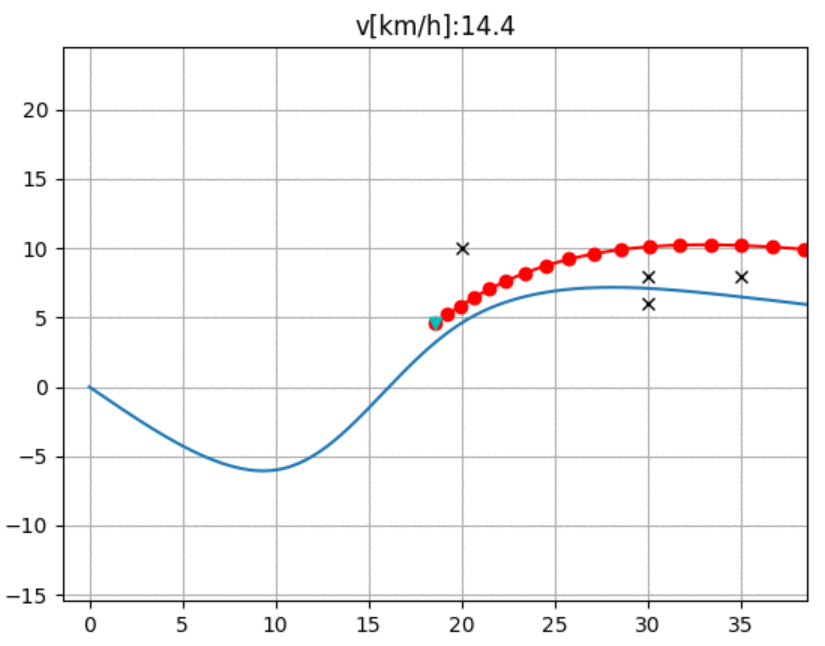
\includegraphics[width=0.5\linewidth]{images/frenet_frame_local_path.png}
    \caption{Fren\'et-Frame path planning, with reference path and local path illustrated. Reproduced from Sakai et al. \cite{sakaiPythonRoboticsPythonCode2018})}
    \label{fig:frenet_frame_local_path}
\end{figure}

\subsubsection{Local Algorithms}
Local algorithms only consider obstacles currently in the proximity of the wheelchair,
and use this information to set the current speed and direction of the wheelchair.
VFH+ (vector field histogram) \cite{ulrichVFHReliableObstacle1998} is one example, which
has been applied to wheelchair control algorithms in prior work \cite{tomariEnhancingWheelchairControl2014}.
VFH+ calculates a polar obstacle density histogram around the robot based on the occupancy grid.
The histogram is then binarized, to classify sectors around the robot as either occupied or not occupied.
Next, a masked polar histogram is generated, which excludes paths that are not possible given the robots
turning radius and kinematics. Finally, a safe direction is chosen which is nearest to the users desired direction.
An example binary histogram is shown in \cref{fig:binary_histogram_vfh}; the chosen direction avoids the obstacle in the
desired direction.

An advantage to this algorithm is that it gives the user more fine-grained control over their speed and direction,
rather than planning a path to their assumed goal.
However an issue with VFH+ is that it does not control the wheelchairs speed, and instead only finds a safe direction.
Ideally the wheelchair should slow down if an obstacle is present.

\begin{figure}[bp]
    \centering
    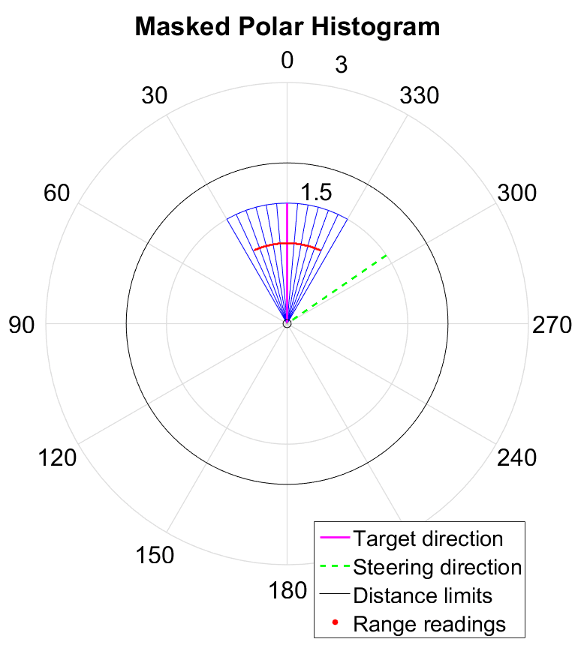
\includegraphics[width=0.4\linewidth]{images/binary_histogram_vfh.png}
    \caption{VFH+ binary histogram, representing direction of obstacles. Reproduced from MathWorks \cite{mathworksVectorFieldHistogram2022})}
    \label{fig:binary_histogram_vfh}
\end{figure}

Another approach to assistive control with local algorithms is haptic feedback. Rather than
blending inputs from the autonomous software and the user, the joystick itself is actuated
to make it more difficult to move in the direction of obstacles \cite{kondoNavigationGuidanceControl2008}\cite{vanderpoortenPoweredWheelchairNavigation2012}.
An advantage of this approach is that it gives the user total control over which direction of movement they choose,
however the additional force required to actuate the joystick may fatigue the user.

%\subsubsection{Path and Trajectory Planning}
%Path planning involves finding a path from the current location to the goal location.

%\subsubsection{Feedback and Control Blending}
%Alternative methods which can be used to provide assistance to the user are haptic feedback and control blending.


% Inputs
% Semi-autonomy
% Full autonomy
% Path Planning
% Obstacle avoidance
% 3D - 2D mapping

% Indoor vs Outdoor assistance.
% Sensors
% Machine Learning
%\cite{tomariEnhancingWheelchairControl2014}
\pagebreak





\section{Methodology}

\subsection{Hardware}
The smart wheelchair should have the ability to sense, process, and manouver within the surrounding environment.
To do this requires some necessary hardware, including a sensor system, compute element, and motor controller.
Due to the 2021-2022 chip shortage, hardware selection was identified as a process that should occur relatively quickly.

The literature review provides a comparison between different sensor types and models. For outdoor navigation assistance,
a forward facing RGB-D camera was selected as the best option for this project - specifically, the Zed 2 Mini.
This was chosen due to the high resolution provided by RGB-D cameras, and the long distance range of the Zed cameras due to 
their passive operation (does not use an IR emitter).

% Should this be in the methodology?
The front of the joystick control unit was selected as the best mounting point for the
stereo camera, due to several reasons:
\begin{enumerate}[topsep=0pt,itemsep=-1ex,partopsep=1ex,parsep=1ex]
    \item Clear view of the environment in front of the wheelchair.
    \item Not obstructed by the user in any wheelchair configuration.
    \item When needed, the user can move the joystick control unit out of the way,
            which also moves the camera out of the way.
\end{enumerate}
However, there are some challenges faced when using this mounting point, which must be addressed.
\begin{enumerate}[topsep=0pt,itemsep=-1ex,partopsep=1ex,parsep=1ex]
    \item Shaky video footage due to low rigidity in joystick mount.
    \item Close to the front of the wheelchair, which reduces visibility of the sides of the wheelchair.
    \item Maximum camera width of \SI{150}{\milli\metre} before doorway manouverability is affected.
\end{enumerate}
Due to the size constraints, the Mini form factor was chosen.

An additional sensor with a wider field of view will be needed for doorway navigation
and wheelchair docking, due to the limitations of this mounting point. The sensor selected for this purpose
was a 2D Lidar unit attached to the base of the wheelchair. However, this sensor will not be used for
our specific application (pathway assistance).

For the compute element, a Nvidia Jetson Xavier NX will be used, due to compatability with the Zed API
and a wide range of ML frameworks, as well as low power use.
The motor controller is being designed by a different thesis student, however will connect with the compute element in a standard way.

\subsection{Dataset Collection}
To train and evaluate machine learning models, a 34 minute driving dataset was collected around Curtin University.
The camera used to collect this dataset was a GoPro Hero 4. Although this camera does lack a depth component,
having a basic dataset for model evaluation is valuable prior to procurement of the RGB-D camera.
% Other datasets

\subsection{Software}
Our software system requires several components. Interaction with the Zed 2 Mini will be done
via the proprietry Stereolabs API, which will provide RGB-D imaging to the computer.
PyTorch \cite{paszkePyTorchImperativeStyle2019} will be used for training and evaluation of machine learning models, as it
provides good compatability with existing models such as YOLOv5 \cite{ultralyticsYOLOv5}
and DeepLabv3 \cite{chenRethinkingAtrousConvolution2017}. OpenCV \cite{bradskiOpenCVLibrary2000} will be used to encode and decode video.
% System diagram
\pagebreak





\section{Current Work}
Part of the current work this semester has included selection of the sensor (Stereolabs Zed 2 Mini) and compute element (Nvidia Jetson),
which has been described in the methodology.
Early identification of viable sensor mounting points on the wheelchair (also described in the methodology) has enabled dataset collection
and algorithm evaluation to progress from an early stage, despite not having access to an RGB-D stereo camera.
Most technical progress this semester has focused on evaluation of various algorithms for scene understanding
and assistive control, as well as writing the software required to evaluate these algorithms.

YOLOv5 \cite{ultralyticsYOLOv5} was one of the first algorithms evaluated for object detection.
The implementation of YOLOv5 includes an inbuilt video encoder and decoder, which simplified
the evaluation process significantly. However, some preprocessing of our video dataset with ffmpeg was required.
YOLOv5 has 5 model sizes (nano, small, medium, large, extra large),
which allow the user to choose between speed and accuracy.
Due to the low latency requirements of a fast moving wheelchair, this algorithm was evaluated using the small model size.

YOLOv5 was evaluated on our Curtin video dataset. As seen in \cref{fig:yolov5s}, this algorithm can identify pedestrians and vehicles with high accuracy.
The confidence of the algorithm decreases when objects are further away, as can be seen with the cars in the background.
YOLOv5 ran in realtime (using a GTX 1080) on the 24 FPS Curtin video dataset.

\begin{figure}[bp]
    \centering
    \includegraphics[width=0.5\linewidth]{images/yolov5s.png}
    \caption{YOLOv5s evaluated on the Curtin dataset}
    \label{fig:yolov5s}
\end{figure}

The next algorithm evaluated was DeepLabv3 \cite{chenRethinkingAtrousConvolution2017}. This is a segmentation algorithm,
which classifies individual pixels within the image rather than drawing bounding boxes around the entire object.
Segmentation algorithms can be more suitable when environment features such as pathways and stairs need to be identified,
as these features do not have well defined bounding boxes.

To evaluate this algorithm, a video encoder and decoder needed to be created. This was done using a Python generator,
so that frames in the video could simply be iterated over within a for loop and only decoded when required.
OpenCV \cite{bradskiOpenCVLibrary2000} was the underlying library used to decode each video frame into a BGR pixel array.
After evaluation of the algorithm, each processed frame was displayed on the screen and encoded into a video file using OpenCV.

Some scene processing algorithms do not run in realtime due to hardware limitations or performance issues.
When this occurs, some frames must be dropped during model evaluation to keep the scene model up to date and minimize latency.
The code used to do this is shown below. By measuring the amount of time taken to process and encode a frame, the current FPS
and number of frames to drop can be calculated.

\begin{lstlisting}[language=Python]
for frame in generate_frame():
    if frames_drop == 0:
        start_time = time.time()
        new_frame = process_frame(frame)
        push_frame(new_frame)
        elapsed = time.time() - start_time
        print(f"Current FPS: {1 / elapsed}")
        frames_drop = math.ceil(elapsed * p.fps) - 1
    else:
        frames_drop -= 1
\end{lstlisting}

To avoid training the model from scratch, a pretrained model is loaded from Pytorch Hub using the code below.
As mentioned in the literature review, image segmentation algorithms can accept different image classifiers as a backbone.
In this case, MobileNetV3 \cite{howardSearchingMobileNetV32019} was used as a backbone due to its fast performance.

\begin{lstlisting}[language=Python]
seg_model = torch.hub.load('pytorch/vision:v0.10.0', 'deeplabv3_mobilenet_v3_large', pretrained=True)
\end{lstlisting}

Another model evaluated was Hybridnet.

The viability of VFH+ was evaluated as an assistive control algorithm. This algorithm was evaluated
in MATLAB using the Navigation toolbox and Lidar toolbox.
First, a virtual 2D environment and occupancy grid were created in MATLAB.
Next, a Lidar 

\pagebreak





\section{Future Work}

\pagebreak





\printbibliography[heading=bibnumbered]

\end{document}
